\section{Deep learning}
Die Begriffe \textit{Deep Learning}, \textit{maschinelles Lernen} und, \textit{künstliche Intelligenz}, werden oft fälschlicherweise auswechselbar verwendet, und in eine Schublade geräumt. Es gibt allerdings eine ganz klare, und für das Verständnis wichtige Hierarchie zwischen den Wörtern. Um Klarheit zu verschaffen werden darum alle Gebiete aufgeführt.

\begin{figure}[hbt]
	\centering
		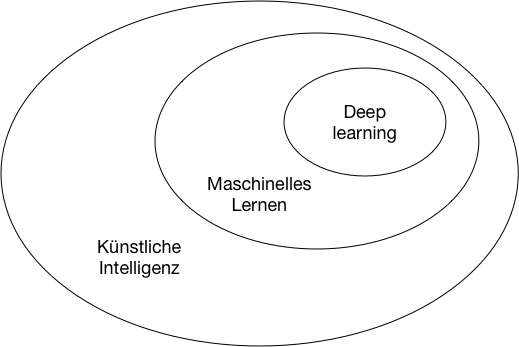
\includegraphics[width=0.6\textwidth]{assets/hierarchy.png}
	\caption{Künstliche Intelligenz, Maschinelles Lernen und Deep Learning}
	\label{img:hierachy}
\end{figure}

Das Gebiet der künstlichen Intelligenz gibt es schon so lange wie den Computer selbst. Die Frage wie schlau ein Computer werden kann, beschäftigt uns bis heute. Al anerkannte Definition für KI gilt, das Bestreben intellektuelle Aufgaben, die normalerweise von Menschen gelöst werden zu automatisieren.

Erste Erfolge erreichte man zum Beispiel mit Schachcomputern, die handgeschriebene Regeln befolgten. Diese Form von künstlicher Intelligenz hatte aber schnell Grenzen, da viele Prozesse schlicht zu komplex waren um sie unter angemessenem Aufwand mit Regeln zu beschreiben. An diesem Punkt wurde man auf maschinelles Lernen aufmerksam.

Der Ablauf von maschinellem Lernen ist grundlegend anders als konventionelles Programmieren. Der Entwickler muss  keinen Programmcode mit festen Regeln schreiben, im Gegenteil. Man liefert dem Computer Eingabe und Ausgabe, und der Computer lernt selber die Regeln. Maschinelles Lernen entstand erst so richtig um 1990, wurde aber schnell zum grössten Teilgebiet der künstlichen Intelligenz.

Beim maschinellem Lernen, lernt die Software im Grunde eine nützlichere Darstellungsweise der Daten bzw. der Eingabe. Anhand dieser anderen Darstellungsweise kann der Computer die Antwort einfach erkennen. Wenn der Computer stufenweise nützlichere Repräsentationen bestimmt kann er zunehmend komplexe Probleme in einfachere Zwischenschritten lösen. Genau das ist deep learning. Es beschreibt also mehr das Konzept von stufenweisem Lernen als eine Methode selber. Ein weit verbreitete Mehode sind allerdings \textit{tiefe künstliche neuronalen Netzen}\parencite[vgl.][]{chollet}.


\subsection{Künstliche Neuronale Netze}
\begin{figure}[hbt]
	\centering
		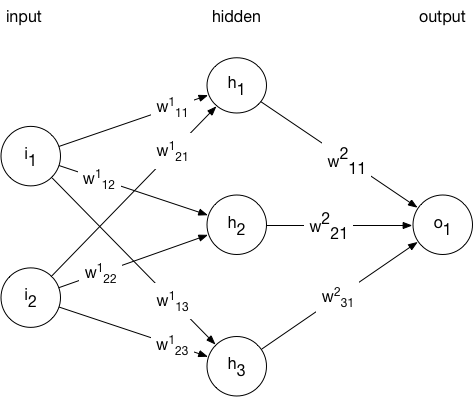
\includegraphics[width=0.6\textwidth]{assets/neural_net.png}
		$$ o_1 = \sigma\Big(\sum_i h_i \cdot w^{2}_{i1}\Big)$$
	\caption{Grafische Darstellung eines künstlichen neuronalen Netzwerks}
	\label{img:neuralnet}
\end{figure}
\textit{Künstliche neuronale Netze} hat man sich, wie der Name schon preisgibt, von der Natur abgesehen. Ähnlich wie in unserem Gehirn gibt es Neuronen (Knoten, z.b $o_1$) und dazwischenliegende Verbindungen. Die Verbindungen haben ein Gewicht $w$. Der Wert eines Knotens ist eine Funktion der Summe all er seiner eingehenden Verbindungen. Diese Funktion wird Aktivierungsfunktion $\sigma$ genannt. Eine bekannte Aktivierungsfunktion ist zum Beispiel die Sigmoid Funktion: $exp(x) = \frac{1}{1+e^{-x}}$\parencite{neuronale_netze}. 
Die Aktivierungsfunktion ist wichtig damit das Netwerk auch nicht lineare Repräsentationen lernen kann. Es ist bewiesen dass solche neuronale Netze jede Funktion abbilden können\parencite[][Kap. 4]{universal}.
\\ \\ 
Die mathematischen Operationen in einem neuronalen Netwerk lassen sich alle als Matrizen-Operationen berechnen. Mit Matrizen kann der Computer auf einer Grafikkarte und mit einem BLAS (\textit{Basic linear algebra system}) sehr effizient rechnen.

\begin{figure}[hbt]
	\centering
		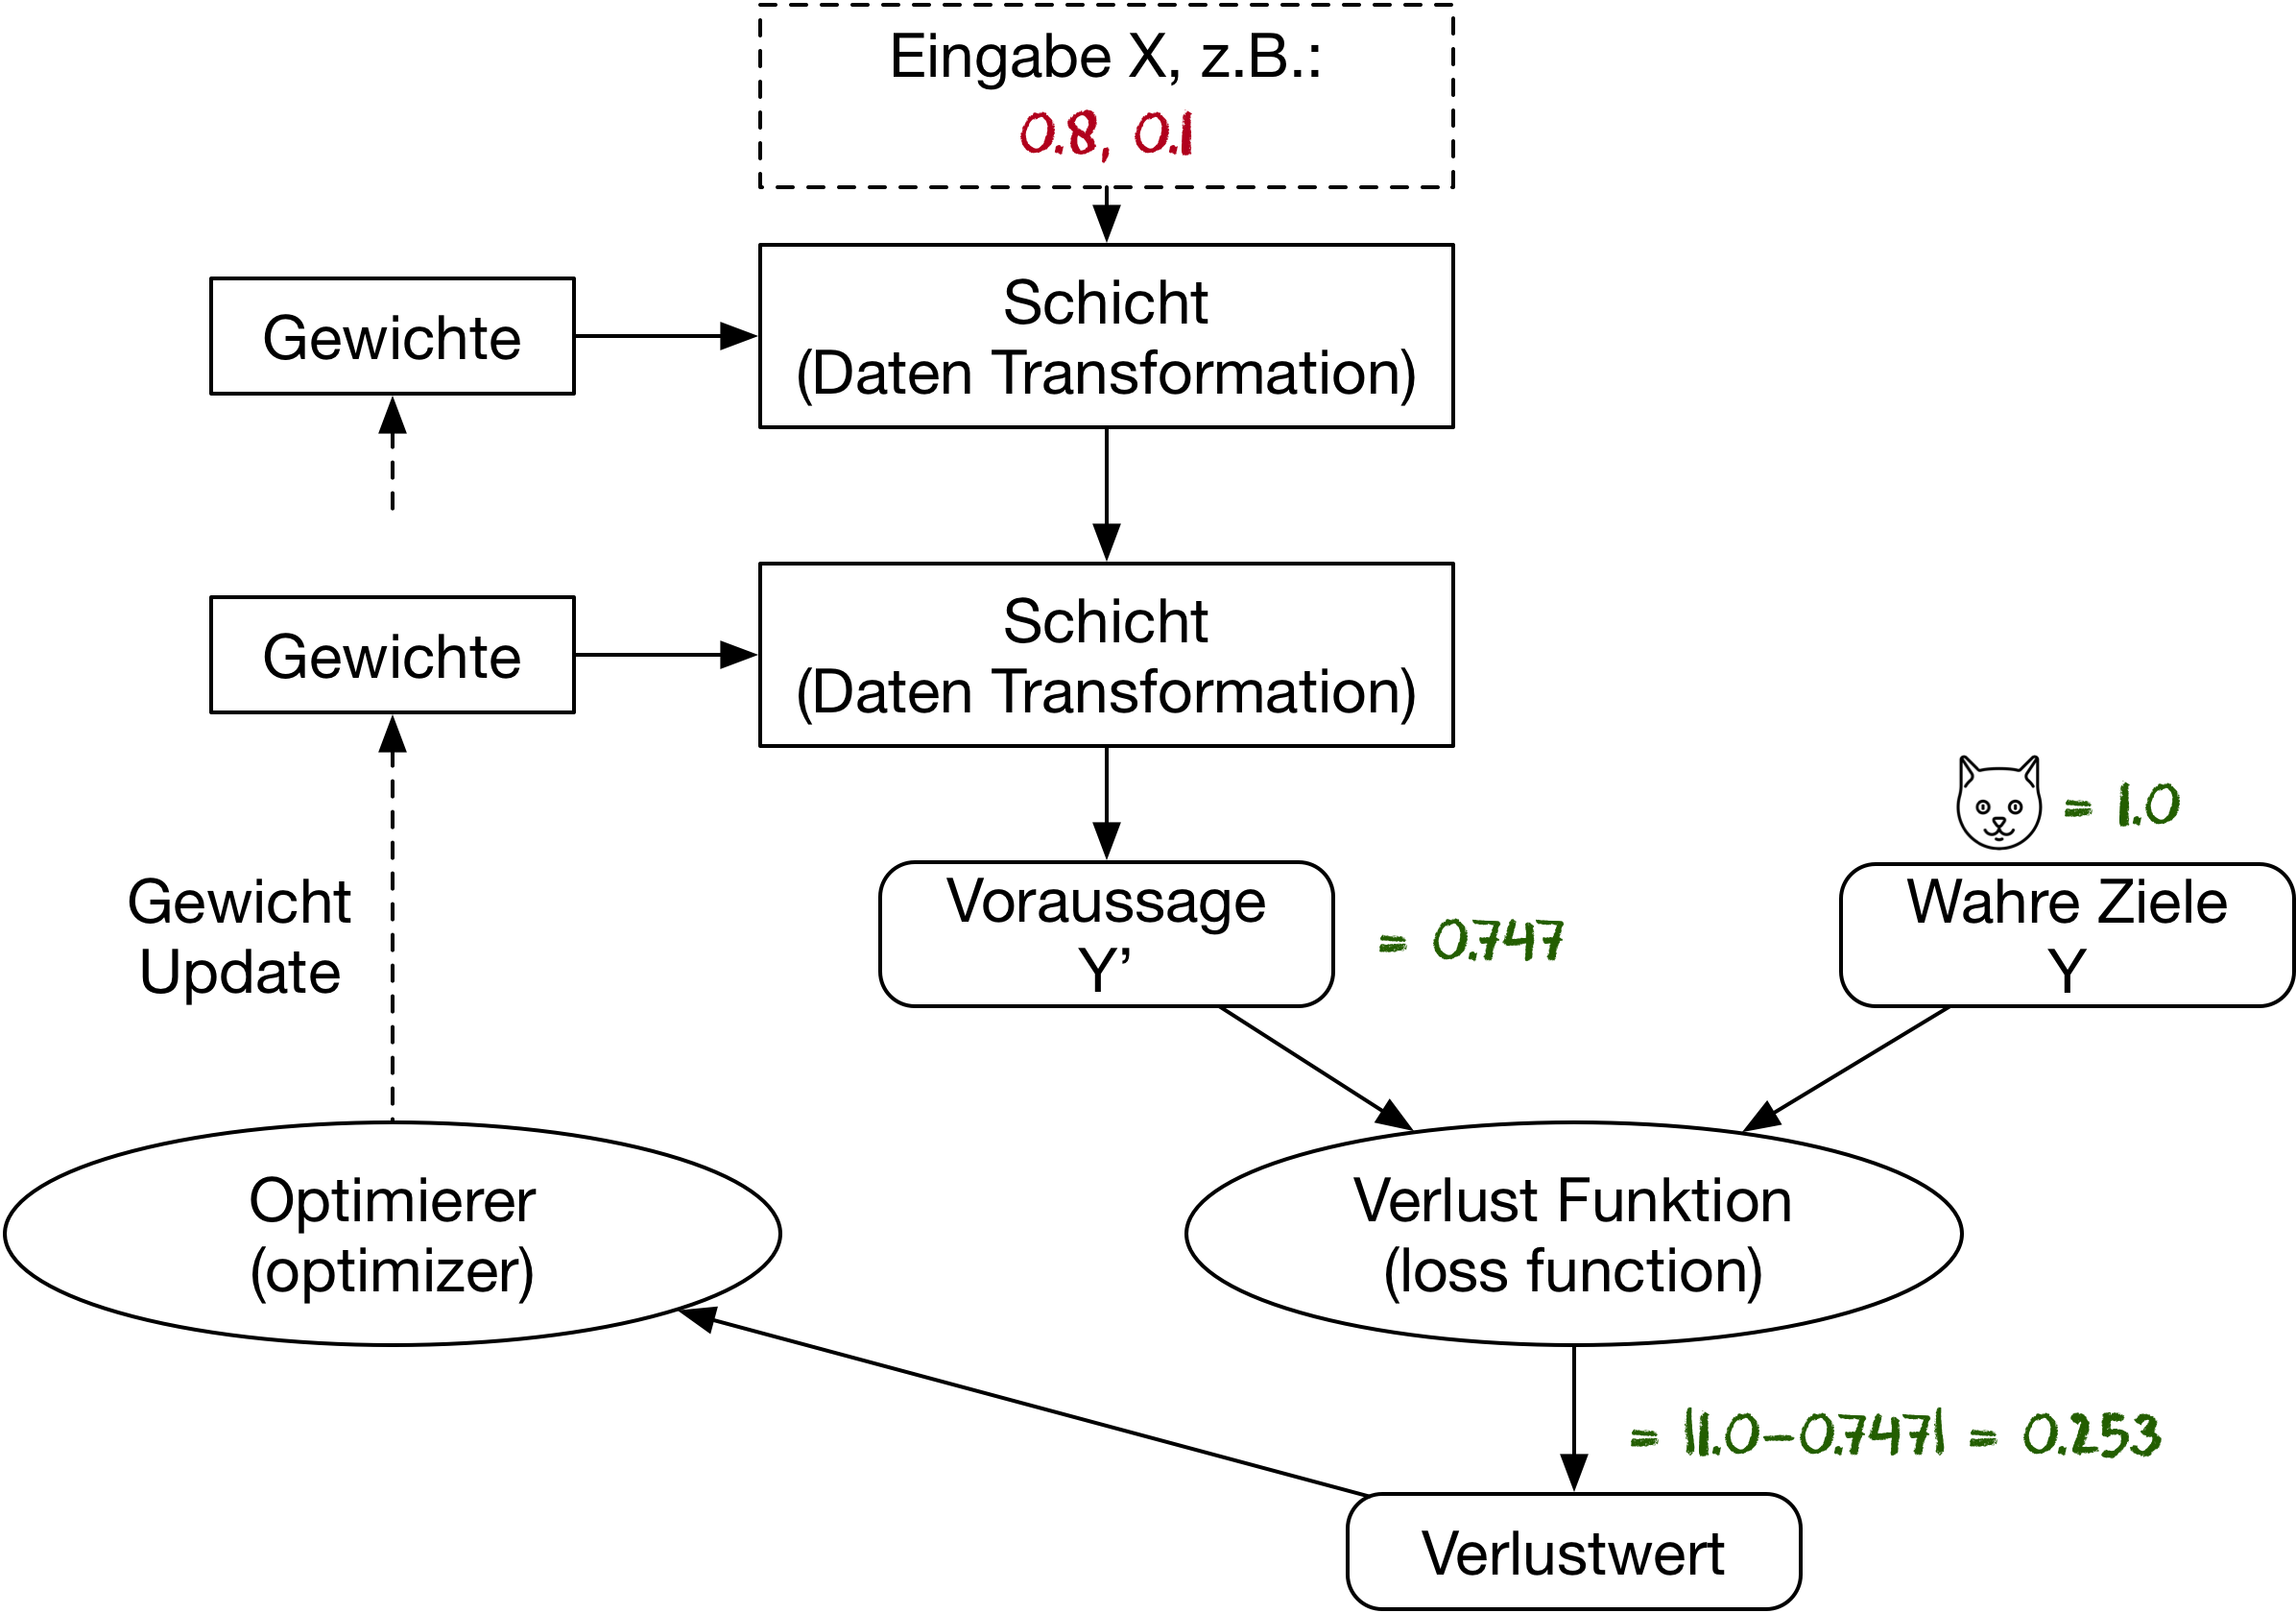
\includegraphics[width=0.6\textwidth]{assets/anatomy.png}
	\caption{Grafische Darstellung eines künstlichen neuronalen Netzwerks}
	\label{img:anatomy}
\end{figure}

Die Gewichte sind die Parameter. Um diese zu erlernen braucht es eine \textit{Verlust Funktion} die uns angiebt, wie weit die Ausgabe von den korrekten Zielen entfernt ist. Anhand des Verlustwerts passt das Netzwerk die Gewichte schrittweise an. Diesen Teil übernimmt der  \textit{Optimierer}. Ein einfacher Optimierer ist zum Beispiel das Gradientenverfahren.
Da bei diesem Typ von neuronalen Netzwerken alle Knoten miteinander verbunden sind, wird es oft \textit{dense neural network} genannt.


\subsection{Convolutional Neural Networks}
\textit{Convolutional Neural Networks} sind eine sehr weit verbreitete Methode im Feld von \textit{Computer Vision}. Der fundamentale Unterschied zwischen dem oben besprochenen \textit{dense network} und einem \textit{CNN} ist, dass ein \textit{CNN} lokale Muster erkennen kann, wo hingegen das vorherige Netzwerk nur globale Muster erkennen konnte. Das heisst, dass ein Muster an einer bestimmten Stelle angetroffen wird, an jeder anderen Stelle ebenfalls erkannt wird. \parencite{chollet}
\begin{figure}[hbt]
	\centering
		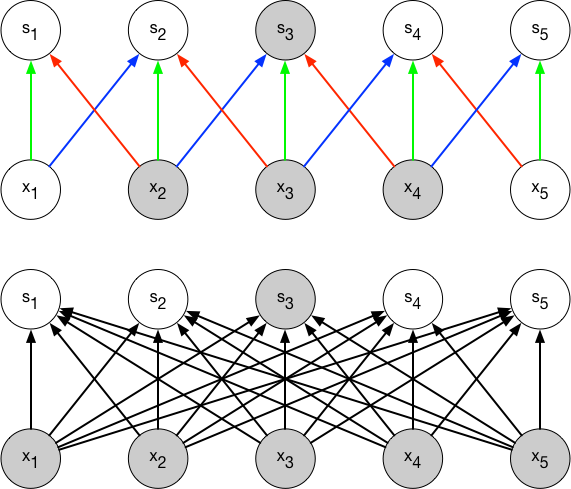
\includegraphics[width=0.6\textwidth]{assets/conv_1d.png}
	\caption{(\textit{Oben})1D Convolution mit \textit{kernel} der Grösse 3. $s_3$ wird durch 3 inputs beeinflusst.
		     (\textit{Unten}) \textit{Dense Network}. $s_3$ wird durch alle inputs beeinflusst.\parencite{goodfellow}}
	\label{img:conv}
\end{figure}

Ein weiterer Vorteil von \textit{Convolutional neural networks} ist, dass sie eine räumliche hyrarchie von Mustern erlernen können. Wenn die Eingabe das Bild einer Katze ist, wird zum Beispiel die erste Schicht unterschiedliche Kanten erkennen, die zweite Schicht dann einzelne Merkmale (z.b Augen), und so weiter.

Damit das gilt, muss aber der analysierte Bereich eines Knotens, von Schicht zu Schicht grösser werden. Deshalb wird meisten nach jedem \textit{convolution layer} ein \textit{pooling layer} gesetzt. Das \textit{pooling layer} fasst mehrere Datenpunkte zusammen um dem nächsten Netzwerk eine grösseren Analysebereich zu verschaffen.
\begin{figure}[hbt]
	\centering
		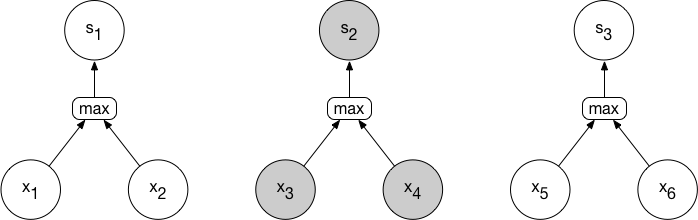
\includegraphics[width=0.6\textwidth]{assets/pooling_1d.png}
	\caption{Abbildung eines 1D Max-Pooling layer. $s_2$ ist $\max (x3, x4)$}
	\label{img:pool}
\end{figure}


\subsection{Recurrent Neural Networks}
\subsection{[andere Tricks]}